\documentclass[arhiv]{../izpit}
\usepackage{fouriernc}
\usepackage{censor}
\usepackage{paralist}
\usepackage{listings}
\usepackage{changepage}
\usepackage{paralist}
\usepackage{amssymb}
\usepackage{subfigure}
\usepackage{url}
\usepackage{tikz}
\usetikzlibrary{calc}
\usetikzlibrary{shapes}

\begin{document}

\izpit{Programiranje I: 2.\ izpit}{29.\ rožnika leta Gospodovega 2015}{
  Čas reševanja je 150 minut.
  Doseženih 100 točk šteje za maksimalno oceno.
  Veliko uspeha!
}

%%%%%%%%%%%%%%%%%%%%%%%%%%%%%%%%%%%%%%%%%%%%%%%%%%%%%%%%%%%%%%%%%%%%%%
\naloga[Igra v petkotniku, 20 + 10 točk]

Stanko se igra nenavadno igro. V oglišča petkotnika zapiše cela števila, katerih vsota je strogo pozitivna. Vsako potezo izbere neko
negativno število $t$ in ga spremeni v $-t$, številoma v obeh sosednjih ogliščih pa prišteje $t$. Pri tej operaciji se skupna vsota števil ohranja.
Slika~\ref{fig:slika1} prikazuje eno od možnih zaporedij treh potez.

\begin{figure}[!h]
\centering
\subfigure[Začetni petkotnik]{
\begin{tikzpicture}
\def\stevilke{{1,4,-1,-3,2}}
\node at (-1.5,0) {};
\node at (1.5,0) {};
\pgfmathsetmacro{\k}{360 / 5};
\foreach \i in {0,...,4} {
  \pgfmathtruncatemacro{\s}{\stevilke[\i]};  
  \node (a_\i) at (90+\i*\k:1) {\s};
}
\foreach \i in {0,...,4} {
  \pgfmathtruncatemacro{\j}{mod(\i+1, 5)};
  \draw (a_\i) -- (a_\j);
}
\end{tikzpicture}
}
\quad
\subfigure[Stanje po 1.\ potezi]{
\begin{tikzpicture}
\def\stevilke{{1,3,1,-4,2}}
\node at (-1.5,0) {};
\node at (1.5,0) {};
\pgfmathsetmacro{\k}{360 / 5};
\foreach \i in {0,...,4} {
  \pgfmathtruncatemacro{\s}{\stevilke[\i]};  
  \node (a_\i) at (90+\i*\k:1) {\s};
}
\foreach \i in {0,...,4} {
  \pgfmathtruncatemacro{\j}{mod(\i+1, 5)};
  \draw (a_\i) -- (a_\j);
}
\end{tikzpicture}
}
\quad
\subfigure[Stanje po 2.\ potezi]{
\begin{tikzpicture}
\def\stevilke{{1,3,-3,4,-2}}
\node at (-1.5,0) {};
\node at (1.5,0) {};
\pgfmathsetmacro{\k}{360 / 5};
\foreach \i in {0,...,4} {
  \pgfmathtruncatemacro{\s}{\stevilke[\i]};  
  \node (a_\i) at (90+\i*\k:1) {\s};
}
\foreach \i in {0,...,4} {
  \pgfmathtruncatemacro{\j}{mod(\i+1, 5)};
  \draw (a_\i) -- (a_\j);
}
\end{tikzpicture}
}
\quad
\subfigure[Stanje po 3.\ potezi]{
\begin{tikzpicture}
\def\stevilke{{1,0,3,1,-2}}
\node at (-1.5,0) {};
\node at (1.5,0) {};
\pgfmathsetmacro{\k}{360 / 5};
\foreach \i in {0,...,4} {
  \pgfmathtruncatemacro{\s}{\stevilke[\i]};  
  \node (a_\i) at (90+\i*\k:1) {\s};
}
\foreach \i in {0,...,4} {
  \pgfmathtruncatemacro{\j}{mod(\i+1, 5)};
  \draw (a_\i) -- (a_\j);
}
\end{tikzpicture}
}
\caption{Potek igre v petkotniku}
\label{fig:slika1}
\end{figure}

\noindent Stanko domneva, da se ta igra vselej konča. Nekajkrat je poskusil in vedno se je zgodilo, da je petkotnik po končno korakih ostal brez negativnih števil.
Svojo hipotezo bi rad preveril še na nekaterih drugih začetnih podatkih. Ker je to zamudno opravilo, potrebuje računalniško podporo.
% \vspace{\baselineskip}

\podnaloga[20 točk]
V \emph{Mathematici} sestavite funkcijo \texttt{igra[l\_]}, ki kot argument dobi začetno stanje igre, tj.\ seznam s petimi elementi. Elementi seznama so števila v ogliščih petkotnika, kot si sledijo v nasprotni smeri urinega kazalca. Prvi in zadnji element seznama sta tudi sosedna. (Predpostavite, da bodo elementi seznama vedno cela števila, njihova vsota pa bo strogo pozitivna.) Funkcija naj vrne seznam, ki vsebuje vsa stanja igre, od začetnega do končnega. Končno stanje je tisto, pri katerem ni več nobenega negativnega števila. \emph{Funkcija naj operacijo vedno izvede na tistem negativnem številu, ki ima najmanjši indeks (tj.\ najbolj levo negativno število v seznamu).} Primer:
%
\begin{verbatim}
In[1]:= igra[{1, 4, -1, -3, 2}]
Out[1]= {{1, 4, -1, -3, 2}, {1, 3, 1, -4, 2}, {1, 3, -3, 4, -2},
         {1, 0, 3, 1, -2}, {-1, 0, 3, -1, 2}, {1, -1, 3, -1, 1},
         {0, 1, 2, -1, 1}, {0, 1, 1, 1, 0}}
\end{verbatim}


\podnaloga[10 točk]
Mojca trdi, da se v splošnem igra ne ustavi. Meni, da je imel Stanko pač srečo, ker funkcija \texttt{igra} operacijo vselej izvede na najbolj levem negativnem številu v seznamu. Stanko bi rad Mojco prepričal, da se moti. Strategijo izbiranja števil bo spremenil, tako da bo vedno izbral najmanjše število. Sestavite še funkcijo \texttt{igra2[l\_]}, ki naj se od prejšnje funkcije razlikuje le v izbiri števila, na katerem izvede operacijo. Vedno naj izbere najmanjše število. Če je takih števil več, naj naključno izbere enega od njih. Primer:
%
\begin{verbatim}
In[2]:= igra2[{1, 4, -1, -3, 2}]
Out[2]= {{1, 4, -1, -3, 2}, {1, 4, -4, 3, -1}, {1, 0, 4, -1, -1},
         {1, 0, 3, 1, -2}, {-1, 0, 3, -1, 2}, {-1, 0, 2, 1, 1},
         {1, -1, 2, 1, 0}, {0, 1, 1, 1, 0}}
         
In[3]:= igra2[{1, 4, -1, -3, 2}]
Out[3]= {{1, 4, -1, -3, 2}, {1, 4, -4, 3, -1}, {1, 0, 4, -1, -1},
         {0, 0, 4, -2, 1}, {0, 0, 2, 2, -1}, {-1, 0, 2, 1, 1},
         {1, -1, 2, 1, 0}, {0, 1, 1, 1, 0}}
\end{verbatim}

%%%%%%%%%%%%%%%%%%%%%%%%%%%%%%%%%%%%%%%%%%%%%%%%%%%%%%%%%%%%%%%%%%%%%%
\naloga[Nanocevke, 30 točk]

V \emph{Mathematici} sestavite funkcijo \texttt{nanocevka[n\_]}, ki nariše ``nanocevko'' dolžine $n$, kot vidite na primerih:
\begin{center}
\begin{tabular}{c@{\hspace{1.5cm}}c@{\hspace{1.5cm}}c}
 
\includegraphics[width=4cm]{cevka0.pdf}&
 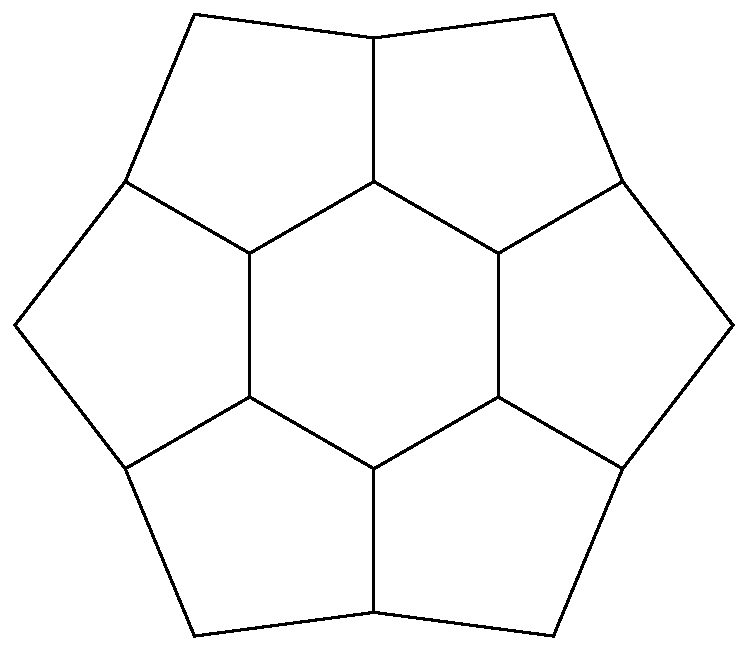
\includegraphics[width=4cm]{cevka1.pdf}&
 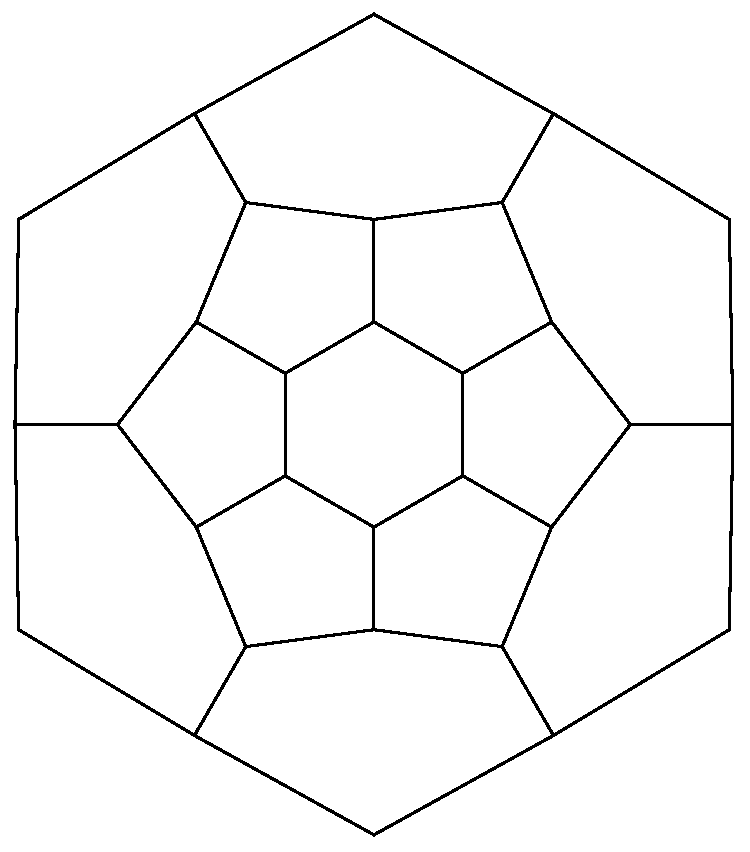
\includegraphics[width=4cm]{cevka2.pdf}\\
  \texttt{nanocevka[0]} &
  \texttt{nanocevka[1]} &
  \texttt{nanocevka[2]}
\end{tabular}
\end{center}

\noindent Nanocevka dolžine 0 je pravilni šestkotnik (glejte sliko na levi), katerega oglišča ležijo na krožnici s polmerom 2. Najvišje ležeče oglišče ima koordinati $(0, 2)$.

Nanocevko dolžine 1 dobimo tako, da nanocevki dolžine 0 dodamo dvanajstkotnik. Njegova oglišča naj ležijo izmenično na krožnicah s polmeroma 4 in 5.
Tista oglišča dvanajstkotnika, ki ležijo na manjši od obeh krožnic, povežemo s pripadajočimi oglišči šestkotnika (kot kaže slika na sredini).

Nanocevko dolžine 2 dobimo tako, da nanocevki dolžine 1 dodamo dvanajstkotnik. Njegova oglišča naj ležijo izmenično na krožnicah s polmeroma 7 in 8.
Oglišča novonastalega dvanajstkotnika, ki ležijo na manjši od obeh krožnic, povežemo s tistimi oglišči prejšnjega dvanajstkotnika, ki ležijo na večji od obeh krožnic (kot kaže slika na desni).

Nanocevko dolžine $n \geq 2$ dobimo tako, da nanocevki dolžine $n-1$ dodamo dvanajstkotnik. Njegova oglišča naj ležijo izmenično na krožnicah s polmeroma $3n+1$ in $3n+2$.
Oglišča novonastalega dvanajstkotnika, ki ležijo na manjši od obeh krožnic, povežemo s tistimi oglišči prejšnjega dvanajstkotnika, ki ležijo na večji od obeh krožnic.


\begin{center}
\begin{tabular}{c}
 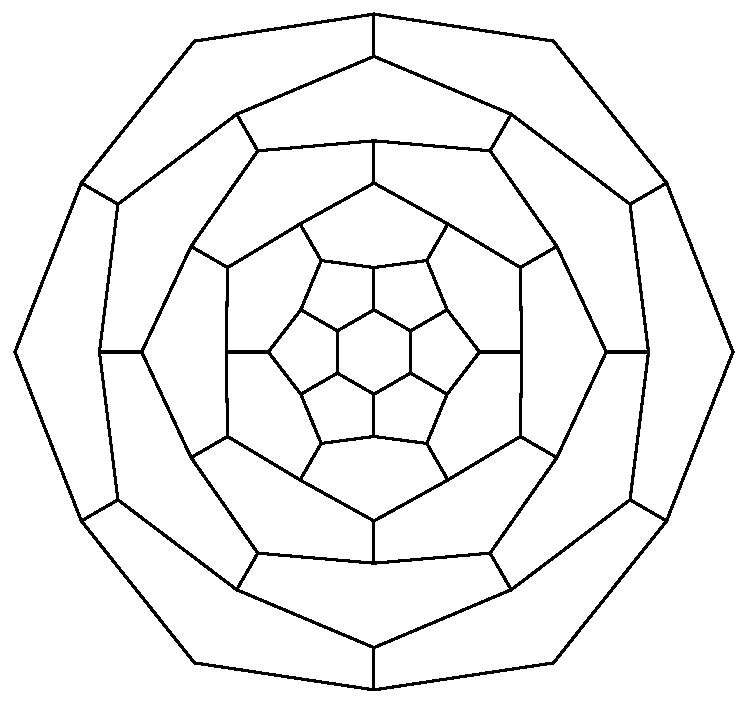
\includegraphics[width=7cm]{cevka5.pdf}\\
  \texttt{nanocevka[5]}
\end{tabular}
\end{center}

%%%%%%%%%%%%%%%%%%%%%%%%%%%%%%%%%%%%%%%%%%%%%%%%%%%%%%%%%%%%%%%%%%%%%%
\naloga[Odločitvena drevesa, 10 + 10 + 10 točk]

% \begin{adjustwidth}{3em}{3em}
% \emph{Zima bleda starka je snega nasula,\\
% drevju bele čevlje zopet je obula,\\
% z belo je preprogo travnik pogrnila,\\
% a veseli potok ves leden molči.} --- Čuki, Sankaška polka
% \end{adjustwidth}
% \vspace{0.5\baselineskip}

% - liha: sin, sinh
%- soda: cos, cosh
%- omejena
%- periodična
%- padajoča
%- naraščajoča
%- monotona
%
%tan, cot, arctan, arccot
%
%omejena:
%  - da:
%    periodična:
%      - da:
%        lihost:
%          - ne: cos,
%          - da: sin,
%      - ne: arctan
%  - ne:
%    - sodost:
%        - da: cosh,
%        - ne:
%        - periodičnost:
%          - ne: sinh,
%          - da: tan
%
%

Dan je razred \texttt{Drevo}, ki predstavlja \emph{odločitveno drevo}. Primer takšnega drevesa je na spodnji sliki:
$$
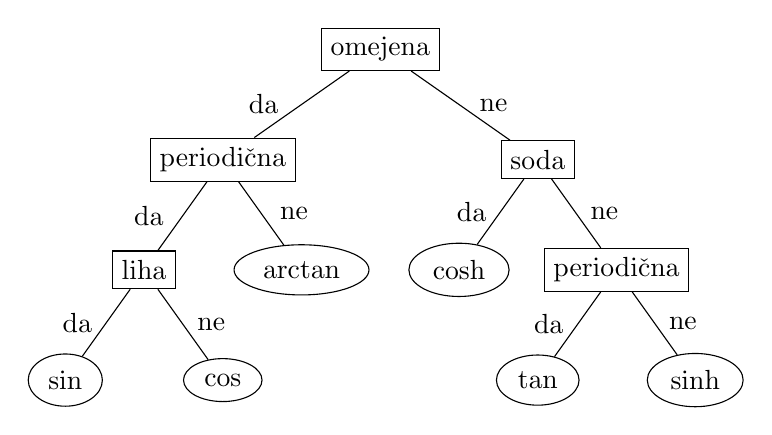
\begin{tikzpicture}[level distance=1.4cm,
    level 1/.style={sibling distance=4.0cm},
    level 2/.style={sibling distance=2cm},
    level 3/.style={sibling distance=2cm}
    ]
    \node[rectangle, draw] (d) {omejena}
      child {node[rectangle, draw] {periodična}
        child {node[rectangle, draw] {liha}
          child { node[ellipse,draw] {$\sin$}
            edge from parent node [left] {da\,}
          }
          child { node[ellipse,draw] {$\cos$}
            edge from parent node [right] {\,ne}
          }
          edge from parent node [left] {da\ \ }
        }
        child {node[ellipse, draw] {$\arctan$}
          edge from parent node [right] {\ ne}
        }
        edge from parent node [left] {da\ \,}
      }
      child {node[rectangle, draw] {soda}
        child { node[ellipse, draw] {$\cosh$}
          edge from parent node [left] {da\,}
        }
        child { node[rectangle, draw] {periodična}
          child { node[ellipse, draw] {$\tan$}
            edge from parent node [left] {da\,}
          }
          child { node[ellipse, draw] {$\sinh$}
            edge from parent node [right] {\,ne}
          }
          edge from parent node [right] {\,ne}
        }
        edge from parent node [right] {\ ne}
      }; 
  \end{tikzpicture}
$$

V našem primeru smo klasificirali funkcije $\sin$, $\cos$, $\tan$, $\arctan$, $\sinh$ in $\cosh$ glede na njihove lastnosti (omejenost, periodičnost ipd.). Tem lastnostim bomo rekli \emph{značilnosti}. Omejili se bomo na takšne značilnosti, ki imajo le dve možni vrednosti: \texttt{True} in \texttt{False}.
Vozlišča drevesa so lahko \emph{notranja} ali pa \emph{listi} (atribut \verb+list+).

Če je vozlišče notranje ($\texttt{list} = \texttt{False}$), ima vozlišče še atribut \texttt{znacilnost}, tj.\ niz z oznako značilnosti, ter atributa \texttt{da} in \texttt{ne}, ki predstavljata usrezni poddrevesi. Če je vozlišče list, ima še atribut \texttt{odgovor}, ki vsebuje ime objekta z ustreznimi značilnostmi (v našem primeru ime funkcije), lahko pa ima tudi vrednost \texttt{None}.

Konstruktor je že implementiran. Zgornje drevo sestavimo takole:
\begin{verbatim}
d = Drevo('omejena', da=Drevo('periodična', da=Drevo('liha', da=Drevo('sin'),
ne=Drevo('cos')), ne=Drevo('arctan')), ne=Drevo('soda', da=Drevo('cosh'),
ne=Drevo('periodična', da=Drevo('tan'), ne=Drevo('sinh'))))
\end{verbatim}
%\begin{verbatim}
%d = Drevo('omejena',
%          da=Drevo('periodična',
%                   da=Drevo('liha', da=Drevo('sin'), ne=Drevo('cos')),
%                   ne=Drevo('arctan')),
%          ne=Drevo('soda',
%                   da=Drevo('cosh'),
%                   ne=Drevo('periodična', da=Drevo('tan'), ne=Drevo('sinh'))))
%\end{verbatim}

\podnaloga[10 točk]
Sestavite metodo \texttt{najdi(self, slovar)}, ki v drevesu poišče in vrne objekt z danimi značilnostmi, ki so shranjene v slovarju \texttt{slovar}. Če objekta ne moremo določiti (ker v slovarju manjka ustrezna značilnost), naj metoda vrne \texttt{None}. Primer (če \texttt{d} ustreza zgornjemu drevesu):
%
\begin{verbatim}
>>> d.najdi({'omejena': True, 'periodična': True, 'liha': True, 'lepa': True})
'sin'
>>> d.najdi({'omejena': False, 'periodična': True, 'soda': True})
'cosh'
>>> print(d.najdi({'periodična': True, 'soda': False, 'liha': True}))
None
\end{verbatim}

\podnaloga[10 točk]
Sestavite metodo \texttt{objekti\_znacilnosti(self)}, ki vrne urejeni par dveh množic. Prva naj vsebuje vse objekte, ki se nahajajo v drevesu, druga pa oznake vseh uporabljenih značilnosti. Primer:
%
\begin{verbatim}
>>> d.objekti_znacilnosti()
({'sin', 'sinh', 'arctan', 'cosh', 'cos', 'tan'},
 {'periodična', 'soda', 'omejena', 'liha'})
\end{verbatim}

\podnaloga[10 točk]
Sestavite metodo \texttt{znacilnosti(self, objekt)}, ki v drevesu poišče podani objekt in vrne slovar njegovih značilnosti. Če objekta ni v drevesu, naj vrne \texttt{None}. Drevo bo vedno takšno, da se noben objekt ne bo pojavil več kot enkrat. Primer:
%
\begin{verbatim}
>>> d.znacilnosti('cosh')
{'soda': True, 'omejena': False}
>>> print(d.znacilnosti('log'))
None
\end{verbatim}


%%%%%%%%%%%%%%%%%%%%%%%%%%%%%%%%%%%%%%%%%%%%%%%%%%%%%%%%%%%%%%%%%%%%%%
\naloga[Nginx, 15 + 15 točk]

Nginx je odprtokodni spletni strežnik, ki je na drugem mestu glede na priljubljenost (na prvem mestu je Apache). Tako kot vsak drug spletni strežnik tudi Nginx vodi dnevnik dostopa (angl.\ access log). Ko uporabnik obišče neko spletno stran, brskalnik pošlje strežniku zahtevek. Strežnik se na zahtevek ustrezno odzove (po navadi tako, da posreduje vsebino spletne strani). Vsak tak dogodek strežnik zabeleži in sicer zapiše v dnevnik eno vrstico besedila oblike:

\begin{verbatim}
$remote_addr - $remote_user [$time_local] "$request" $status $body_bytes_sent
"$http_referer" "$http_user_agent"
\end{verbatim}

\noindent Zgled (iz dnevnika strani \url{http://upm.putka.si}):

\begin{verbatim}
84.20.241.170 - - [15/Nov/2014:10:31:15 +0000] "GET /tasks/2014/ HTTP/1.1" 200
1599 "http://putka.upm.si/tasks/" "Mozilla/5.0 (Windows NT 6.1; WOW64)
AppleWebKit/537.36 (KHTML, like Gecko) Chrome/38.0.2125.111 Safari/537.36"
\end{verbatim}

\noindent Iz zapisa se da razbrati, da je uporabnik z IP naslovom 84.20.241.170 dne 15.\ 11.\ 2014 ob 10:31:15 zahteval vsebino strani \url{/tasks/2014/} (oz.\ \url{http://putka.upm.si/tasks/2014/}). Strežnik je posredoval 1599 bajtov dolg odgovor s statusno kodo 200 (vse OK). Da se še razbrati, da je do te strani prišel preko povezave na \url{http://putka.upm.si/tasks/} in da je uporabljal brskalnik Chrome na operacijskem sistemu Windows 7.

\vspace{0.5\baselineskip}
\noindent Še en zgled:

\begin{verbatim}
74.208.16.114 - - [15/Nov/2014:10:44:45 +0000] "POST /wp-login.php HTTP/1.1" 404
1650 "http://www.google.com/" "Opera/9.80 (Windows NT 6.1; WOW64)
Presto/2.12.388 Version/12.14"
\end{verbatim}

\noindent Iz zapisa se da razbrati, da se je nepridiprav iz ZDA poskušal prijaviti v spletno stran, pri čemer je predpostavil, da gre za WordPress blog.
Ker pa v tem primeru ne gre za WordPress blog (datoteka \url{wp-login.php} na strežniku ne obstaja),
se je strežnik odzval s statusno kodo 404 (strani ni mogoče najti).

%\podnaloga[20 točk]
%Kakšna je časovna zahtevnost algoritma iz prejšnje točke? Utemeljite.

\podnaloga[15 točk]
Napišite funkcijo \texttt{beri\_log(ime\_datoteke)}, ki kot argument dobi niz z imenom datoteke in vrne seznam naborov, kjer vsak nabor ustreza eni vrstici dnevnika. Vsak nabor naj vsebuje 8 elementov, pri čemer naj bo:
\begin{compactitem}
\item IP naslov tipa \texttt{IPv4Address} (iz modula \texttt{ipaddress});
\item časovna oznaka naj bo tipa \texttt{datetime} (iz modula \texttt{datetime});
\item statusna koda in velikost naj bosta celi števili (tip \texttt{int});
\item ostali podatki pa naj bodo nizi.
\end{compactitem}

\vspace{0.5\baselineskip}
\noindent Primer (če datoteka access.log vsebuje zgornji dve vrstici):
%
\begin{verbatim}
>>> beri_log('access.log')
[(IPv4Address('84.20.241.170'), '-', datetime.datetime(2014, 11, 15, 10, 31, 15,
tzinfo=datetime.timezone.utc), 'GET /tasks/2014/ HTTP/1.1', 200, 1599,
'http://putka.upm.si/tasks/', 'Mozilla/5.0 (Windows NT 6.1; WOW64)
AppleWebKit/537.36 (KHTML, like Gecko) Chrome/38.0.2125.111 Safari/537.36'),
(IPv4Address('74.208.16.114'), '-', datetime.datetime(2014, 11, 15, 10, 44, 45,
tzinfo=datetime.timezone.utc), 'POST /wp-login.php HTTP/1.1', 404, 1650,
'http://www.google.com/', 'Opera/9.80 (Windows NT 6.1; WOW64) Presto/2.12.388
Version/12.14')]
\end{verbatim}

\noindent\emph{Nasvet:}
\verb+datetime.datetime.strptime(casovna_oznaka, '%d/%b/%Y:%H:%M:%S %z')+

\podnaloga[15 točk]
Napišite funkcijo \texttt{statistika(seznam)}, ki kot argument dobi seznam naborov, kot ga vrne prejšnja funkcija. Prešteje naj število zahtevkov glede na IP in statusno kodo. Vrne naj slovar, kjer so ključi IP naslovi, vrednosti pa slovarji, ki imajo za ključe statusne kode, pripadajoče vrednosti pa so frekvence vrstic s to kombinacijo IP naslova in statusne kode. Primer:
\begin{verbatim}
>>> statistika(beri_log('access.log'))
{ipaddress.IPv4Address('74.208.16.114'): {404: 1},
 ipaddress.IPv4Address('84.20.241.170'): {200: 1}}
\end{verbatim}


\end{document}
